\chapter{Il servizio di Help Desk}\label{ch:servizio_helpdesk}

	% TODO tenere in mente non di descrivere i servizi all'interno del capitolato ma di spiegare come si vanno ad implementare, prendere spunto da gobbo

	L'azienda \azienda, in base agli obiettivi descritti all'interno del capitolato fornito dall'\istituto~Ortopedico Gaetano Pini, stabilisce a sua volta una serie di obiettivi per il \rollout~del nuovo servizio di \helpdesk.
	
	Questi vengono posti con lo scopo di erogare un servizio \textit{misurabile}, assicurando al cliente \textit{alta qualità} e guidando il progetto con \textit{logiche di efficienza ed efficacia}.
	% , come descritto successivamente in ??
	
\section{Lo scopo dell'\helpdesk}\label{sec:scopo_helpdesk}
	
	L'\helpdesk~aziendale è un asset tattico e fondamentale in quanto fornisce un ``\textit{single point of contact}'' (\textit{SPOC}) per gli utenti, ovvero permette di unificare il servizio in un singolo punto centrale.

	Lo scopo principale è quello di fornire aiuto e supporto immediati agli utenti per quanto riguarda i problemi di natura tecnica.
	Questo può fare parte di una infrastruttura informatica aziendale più ampia nella quale sono presenti altri servizi che hanno come scopo creare una struttura organizzata dei servizi volti agli utenti.
	
	Come altri \helpdesk~aziendali, anche quello che viene progettato per l'\istituto~assicura servizi che sono disegnati sulla realtà specifica e dedicati a quest'ultimo.
	
	In Fig. \ref{fig:service-desk-types}~viene rappresentata la struttura generale di un \helpdesk~aziendale, nel quale vi sono un primo, un secondo ed un terzo livello di supporto tecnico all’utente, ciascuno con uno scopo ben preciso:
	% https://www.bmc.com/blogs/support-levels-level-1-level-2-level-3/
	\begin{itemize}[noitemsep]
		\item \textit{\helpdesk~di primo livello}: risoluzione di problemi basilari tramite supporto che non richiede una profonda conoscenza del sistema e dei servizi che lo compongono;
		% Basic help desk resolution and service desk delivery. Support for basic customer issues such as solving usage problems and fulfilling service desk requests that need IT involvement.;
		\item \textit{\helpdesk~di secondo livello}: supporto tecnico che richiede una conoscenza completa del sistema e dei servizi offerti da questo. 
		I problemi che non è possibile risolvere tramite le procedure \textit{prefabbricate} del primo livello, subiscono \textit{escalation} e arrivano al secondo livello;
		% In-depth technical support. Experienced and knowledgeable technicians assess issues and provide solutions for problems that cannot be handled by tier 1.;
		\item \textit{\helpdesk~di terzo livello}: a questo livello tecnici esperti prendono in mano il problema e cercano di risolverlo avendo a loro disposizione tutte le risorse necessarie del sistema.
		% Expert product and service support. Access to the highest technical resources available for problem resolution or new feature creation..
	\end{itemize}

	\begin{figure}[h!]
		\centering
		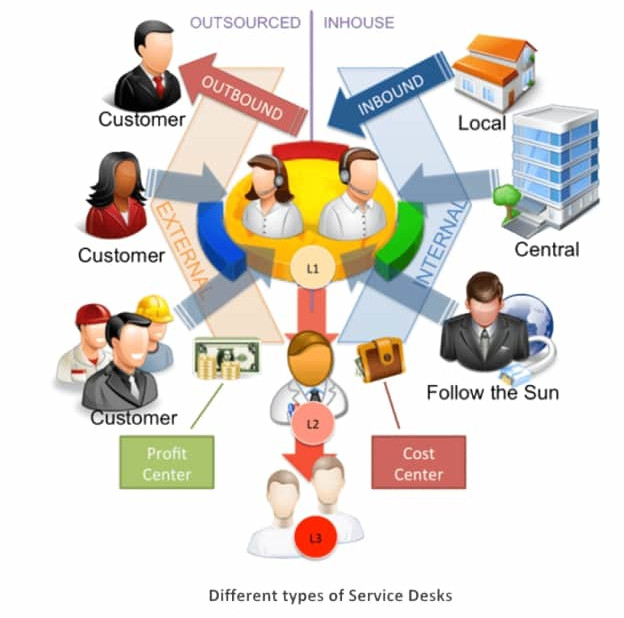
\includegraphics[width=\linewidth]{img/service-desk-types.jpg}
		\caption{``\textit{Service Desk classification}''\cite{service_desk}}
		\label{fig:service-desk-types}
	\end{figure}
	
	\newpage
	
	% preso da petenazzi
	% L'\helpdesk~ha lo scopo di fornire un punto di contatto unificato (\textit{single point of contact}, SPOC), un secondo livello di supporto, e il coordinamento di eventuali fornitori terzi per fornire un terzo livello di supporto.
	
	% https://www.bmc.com/blogs/help-desk-vs-service-desk-whats-difference/
	% The IT help desk is typically seen as more tactical, with the primary goal of helping to quickly resolve end users’ immediate needs and technical issues and incidents. The help desk is reactive in nature, but is expected to be efficient and speedy. The IT help desk can be separate from or part of a larger service desk operation to improve the overall organization’s customer services.

\section{Utenti del servizio}\label{sec:utenti}

	Come descritto nel Capitolato Tecnico dell'istituto, il servizio di \helpdesk~dovrà essere usufruibile da parte di tutto il personale interno dell'azienda e da parte dei clienti, in base alla loro necessità.
	
%	Alcuni esempi di utilizzo da parte degli utenti:
%	\begin{itemize}
%		\item un utente esterno non potrà accedere ai servizi a meno che non sia stato cliente dell'isituto;
%		\item un cliente potrà accedere per vedere solamente i risultati dei servizi di cui ha usufruito;
%		\item gli utenti dell'area amministrativa non potranno avere accesso ad aree come la parte sanitaria e la parte tecnica (server) e viceversa.
%	\end{itemize}

	\subsection{Aree applicative}
	
		\azienda~si impenga, come richiesto dall'\istituto, a implementare i servizi per le seguenti aree applicative:
		\begin{itemize}[noitemsep]
			\item \textit{Area Sanitaria};
			\item \textit{Area Amministrativa};
			\item \textit{Area Direzionale};
			\item \textit{Area Servizi Generali}.
		\end{itemize}
	
		\begin{figure}[h!]
			\centering
			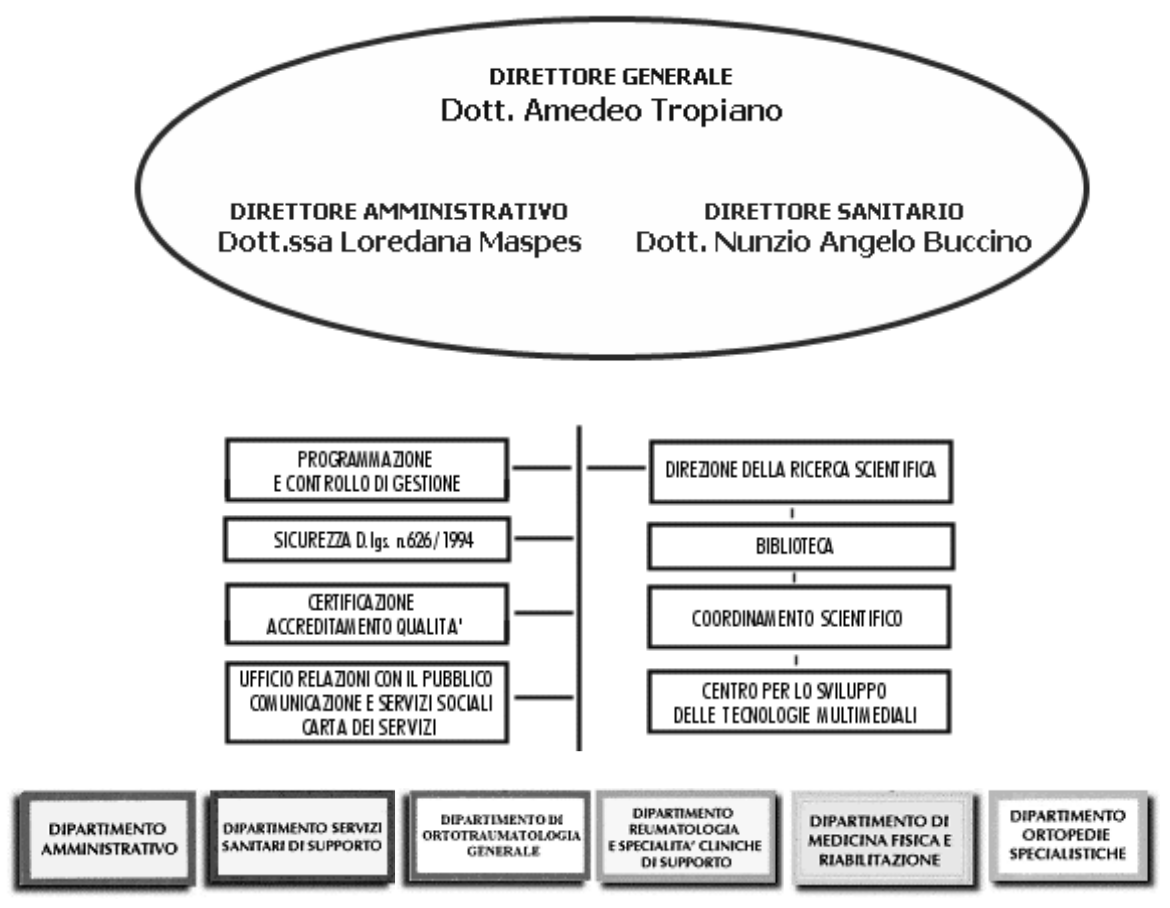
\includegraphics[width=\linewidth]{img/gerarchia.png}
			\caption{Struttura e organizzazione dell'UO Informatico Aziendale}
			\label{fig:gerarchia}
		\end{figure}

		Nel Cap. \ref{ch:implementazione}, viene descritta la modalità di implementazione scelta e come questa avviene per ciascun settore.
		
%\section{Descrizione generale dell’ambiente}\label{sec:ambiente}
%
%	\subsection{Locali fisici dell'ospedale}
%	
%		La descrizione dei locali fisici nei quali è suddiviso l'ospedale si può trovare nel paragrafo 1.1 del capitolato tecnico.

\newpage
\section{Obiettivi del \textit{nuovo} servizio di \helpdesk}\label{sec:obiettivi_helpdesk}

	% Di seguito vengono elencati gli obiettivi che \azienda~ si impegna di rispettare per quanto riguarda il nuovo servizio di \helpdesk, in base a quello che viene richiesto dal \hl{contraente}.
	
	Di seguito vengono elencati gli obiettivi descritti dal \proponente~nel paragrafo 1.2 del capitolato tecnico fornito.
	A ciascuno di questi viene assegnato un identificatore univoco che ne consente una successiva associazione con le attività che \azienda~pianifica di svolgere per portare a termine il progetto.
	
	La classificazione di tali obiettivi permette successivamente di poter verificarne ogettivamente la loro completezza, tramite l'uso di altri parametri, misurandone inoltre la qualità, l'efficacia e l'efficienza.
	
	Gli obiettivi sono dunque presentati in maniera tabulare dove nella prima colonna viene indicato l'identificatore del tipo \textit{IGP\_[NUMERO OBIETTIVO]} (\textit{IGP} come acronimo di \textit{Istituto Gaetano Pini}) e, nella seconda colonna, viene indicato l'obiettivo richiesto.
	
	\newcommand\larghezzacolonnaID{1cm}
	\newcommand\larghezzacolonnaDESC{11cm}

	\begin{table}[H]
		\centering
		\renewcommand\arraystretch{2}
		\begin{tabular}{|>{\raggedright\arraybackslash}m{\larghezzacolonnaID}|m{\larghezzacolonnaDESC}|}
			\hline
			\rowcolor{pantone}
			\multicolumn{1}{|>{\centering\arraybackslash}m{\larghezzacolonnaID}|}{\color{white}\textbf{ID}} &
			\multicolumn{1}{>{\centering\arraybackslash}m{\larghezzacolonnaDESC}|}{\color{white}\textbf{Descrizione}} \\
			\hline
			
			\codiceobiettivo & Ammodernamento organizzativo delle risorse e dei processi, volto al miglioramento della loro efficienza, all’interscambio informativo ed al governo dell’attività aziendale.
			\\\hline
			
			\codiceobiettivo & \vfill Razionalizzazione del sistema informatico e del servizio. \vfill
			\\\hline
			
			\codiceobiettivo & Consolidamento dei sistemi (hw, sw) per avere maggiore facilità di gestione.
			\\\hline
			
			\codiceobiettivo & Riprogettazione del sistema ed evoluzione tecnologica dei componenti dove più obsoleti.
			\\\hline
			
			\codiceobiettivo & Riprogettazione dei servizi generali di continuità, sicurezza, ecc. al fine di avere una architettura più stabile e trasversale ai diversi sistemi.
			\\\hline
						
			\codiceobiettivo & Presa in carico del sistema informativo sia per nuove componenti offerte sia per l’esistente; è lasciata facoltà all’offerente di mantenere gli attuali sistemi, ottimizzandone il funzionamento rispetto ai livelli di servizio richiesti, oppure di procedere alla sostituzione degli stessi. Per quest’ultimo aspetto, l’offerente dovrà farsi carico della completa migrazione delle informazioni gestite.
			\\\hline
					
		\end{tabular}
		\renewcommand\arraystretch{1}
		\caption{Lista obiettivi del nuovo \helpdesk~(pt. 1)}
	\end{table}	

	\begin{table}[H]
		\centering
		\renewcommand\arraystretch{2}
		\begin{tabular}{|>{\raggedright\arraybackslash}m{2cm}|m{10cm}|}
			\hline
			\rowcolor{pantone}
			\multicolumn{1}{|>{\centering\arraybackslash}m{2cm}|}{\color{white}\textbf{ID}} &
			\multicolumn{1}{>{\centering\arraybackslash}m{10cm}|}{\color{white}\textbf{Descrizione}} \\\hline
			
			\codiceobiettivo & Standardizzazione degli ambienti, con adeguamento alle principali normative e standard correnti, assicurando al contempo il mantenimento delle specificità dell’Istituto.
			\\\hline
			
			\codiceobiettivo & Impulso alla dematerializzazione dei documenti scambiati in Istituto e dall’Istituto, con conseguente risparmio sia di materiali (carta) che di tempo.
			\\\hline
			
			\codiceobiettivo & Supporto nei processi di riorganizzazione che l’Istituto che mettendo in atto, quali, ad esempio non esaustivo:
			\begin{itemize}[noitemsep]
				\item passaggio completo a controllo di gestione e budgeting;
				\item unificazione rete imaging;
				\item collegamento tra flussi dei sistemi gestionali sanitari e processi clinici e diagnostici.
			\end{itemize}
			\\\hline
		
			\codiceobiettivo & Progettazione e fornitura di sistemi applicativi che possano essere utilizzati quali base per la successiva introduzione di nuovi servizi innovativi; inoltre, disponibilità a realizzare sperimentazioni di nuovi sistemi.
			\\\hline
			
			\codiceobiettivo & Organizzazione del servizio con interfacce univoche verso la direzione e verso gli utenti.
			\\\hline
			
			\codiceobiettivo & Consolidamento dei servizi di gestione e assistenza, attualmente dispersi tra diversi fornitori, per evitare la frammentazione delle responsabilità.
			\\\hline
			
			\codiceobiettivo & Disponibilità di strumenti di controllo dei livelli di servizio forniti.
			\\\hline
			
			\codiceobiettivo & Disponibilità di strumenti per la registrazione, l’analisi ed il tracciamento delle richieste dell’utenza.
			\\\hline
			
			\codiceobiettivo & La manutenzione, assistenza e gestione dei sistemi attualmente in uso e che si intende mantenere nell’architettura globale, assicurandone l’evoluzione nei prossimi 9 anni.
			\\\hline
			
		\end{tabular}
		\renewcommand\arraystretch{1}
		\caption{Lista obiettivi del nuovo \helpdesk~(pt. 2)}
	\end{table}	
	\begin{table}[H]
		\centering
		\renewcommand\arraystretch{2}
		\begin{tabular}{|>{\raggedright\arraybackslash}m{2cm}|m{10cm}|}
			\hline
			\rowcolor{pantone}
			\multicolumn{1}{|>{\centering\arraybackslash}m{2cm}|}{\color{white}\textbf{ID}} &
			\multicolumn{1}{>{\centering\arraybackslash}m{10cm}|}{\color{white}\textbf{Descrizione}} \\\hline
			
			\codiceobiettivo & La fornitura di nuovi sistemi invece di quelli attualmente in uso e che si intende sostituire, evidenziando il razionale della sostituzione e i vantaggi introdotti con le nuove soluzioni.
			\\\hline
			
			\codiceobiettivo & L’attuazione di un progetto organizzativo, completo di attività di BPR, in grado di supportare efficacemente l’adozione della piattaforma applicativa proposta, tenendo conto delle esigenze e delle specificità dell’Istituto.
			\\\hline
			
			\codiceobiettivo & La fornitura di nuovi sistemi che integrano e si aggiungono a quelli già in uso sia in forma definitiva che di sperimentazione.
			\\\hline
			
			\codiceobiettivo & L’eventuale progettazione e realizzazione dei lavori per la riorganizzazione dei locali CED. Sarà cura dell’offerente definire quali sistemi mantenere nel CED dell’Istituto e quali ospitare presso un proprio centro esterno di servizio adeguatamente collegato per via telematica a spese dell’offerente stesso.
			\\\hline
			
			\codiceobiettivo & La sperimentazione di soluzioni innovative.
			\\\hline
			
			\codiceobiettivo & Tutti i servizi di gestione, manutenzione ed assistenza di tutti i sistemi di cui ai punti precedenti, l’organizzazione del Centro di Gestione Integrato ed i servizi di supporto professionale (direzionale, gestione personale).
			\\\hline
			
			\codiceobiettivo & Evidenzi le capacità progettuali e le competenze dell’offerente descrivendo:
			\begin{itemize}[noitemsep]
				\item un progetto tecnico di proposta per l’Integrazione della Rete Radiologica;
				\item le soluzioni disponibili e le proposte dell’offerente riguardo ai progetti di sperimentazione ed innovazione descritti in dettaglio successivamente o proposti dall’offerente stesso.
			\end{itemize}
			\\\hline
	
		\end{tabular}
		\renewcommand\arraystretch{1}
		\caption{Lista obiettivi del nuovo \helpdesk~(pt. 3)}
	\end{table}	

%	\newpage
%	\begin{itemize}[noitemsep]
%		
%		\item Ammodernamento organizzativo delle risorse e dei processi, volto al miglioramento della loro efficienza, all’interscambio informativo ed al governo dell’attività aziendale;
%		\item Razionalizzazione del sistema informatico e del servizio.
%		\item Consolidamento dei sistemi (hw, sw) per avere maggiore facilità di gestione.
%		\item Riprogettazione del sistema ed evoluzione tecnologica dei componenti dove più obsoleti.
%		\item Riprogettazione dei servizi generali di continuità, sicurezza, ecc al fine di avere una architettura più stabile e trasversale ai diversi sistemi.
%		\item Presa in carico del sistema informativo sia per nuove componenti offerte sia per l’esistente; è lasciata facoltà all’offerente di mantenere gli attuali sistemi, ottimizzandone il funzionamento rispetto ai livelli di servizio richiesti, oppure di procedere alla sostituzione degli stessi. Per quest’ultimo aspetto, l’offerente dovrà farsi carico della completa migrazione delle informazioni gestite.
%		\item Standardizzazione degli ambienti, con adeguamento alle principali normative e standard correnti, assicurando al contempo il mantenimento delle specificità dell’Istituto.
%		\item Impulso alla dematerializzazione dei documenti scambiati in Istituto e dall’Istituto, con conseguente risparmio sia di materiali (carta) che di tempo.
%		\item Supporto nei processi di riorganizzazione che l’Istituto che mettendo in atto, quali, ad esempio non esaustivo,:
%		\begin{itemize}[noitemsep]
%			\item passaggio completo a controllo di gestione e budgeting
%			\item unificazione rete imaging
%			\item collegamento tra flussi dei sistemi gestionali sanitari e processi clinici e diagnostici
%		\end{itemize}
%		\item Progettazione e fornitura di sistemi applicativi che possano essere utilizzati quali base per la successiva introduzione di nuovi servizi innovativi; inoltre, disponibilità a realizzare sperimentazioni di nuovi sistemi.
%		\item Organizzazione del servizio con interfacce univoche verso la direzione e verso gli utenti
%		\item Consolidamento dei servizi di gestione e assistenza, attualmente dispersi tra diversi fornitori, per evitare la frammentazione delle responsabilità
%		\item Disponibilità di strumenti di controllo dei livelli di servizio forniti
%		\item Disponibilità di strumenti per la registrazione, l’analisi ed il tracciamento delle richieste dell’utenza.
%		\item Alle imprese offerenti è richiesto di presentare un progetto che, partendo dall’analisi della situazione esistente presso l’Istituto,
%		
%	\end{itemize}
%	
%	Includa una offerta tecnica ed economica per:
%	
%	\begin{itemize}[noitemsep]
%		
%		\item La manutenzione, assistenza e gestione dei sistemi attualmente in uso e che si intende mantenere nell’architettura globale, assicurandone l’evoluzione nei prossimi 9 anni.
%		\item La fornitura di nuovi sistemi in vece di quelli attualmente in uso e che si intende sostituire, evidenziando il razionale della sostituzione e i vantaggi introdotti con le nuove soluzioni.
%		\item L’attuazione di un progetto organizzativo, completo di attività di BPR, in grado di supportare efficacemente l’adozione della piattaforma applicativa proposta, tenendo conto delle esigenze e delle specificità dell’Istituto.
%		\item La fornitura di nuovi sistemi che integrano e si aggiungono a quelli già in uso sia in forma definitiva che di sperimentazione.
%		\item L’eventuale progettazione e realizzazione dei lavori per la riorganizzazione dei locali CED. Sarà cura dell’offerente definire quali sistemi mantenere nel CED dell’Istituto e quali ospitare presso un proprio centro esterno di servizio adeguatamente collegato per via telematica a spese dell’offerente stesso.
%		\item La sperimentazione di soluzioni innovative, così come descritto in dettaglio nei successivi paragrafi.
%		\item Tutti i servizi di gestione, manutenzione ed assistenza di tutti i sistemi di cui ai punti precedenti, l’organizzazione del Centro di Gestione Integrato ed i servizi di supporto professionale (direzionale, gestione personale) descritti successivamente.
%		\item Evidenzi le capacità progettuali e le competenze dell’offerente descrivendo:
%		\begin{itemize}[noitemsep]
%			\item un progetto tecnico di proposta per l’Integrazione della Rete Radiologica
%			\item le soluzioni disponibili e le proposte dell’offerente riguardo ai progetti di sperimentazione ed innovazione descritti in dettaglio successivamente o proposti dall’offerente stesso.
%		\end{itemize}
%	\end{itemize}

	\newpage
	\subsection{Business Process Re-engineering (BPR)}\label{sec:desc_bpr}
		
		Per ``\textit{Business Process Re-engineering}'' (in italiano ``\textit{riprogettazione dei processi aziendali}'') si intende un intervento organizzativo di profonda revisione dei procedimenti operativi che non risultano più adeguati alle necessità aziendali.
		Come ciascun altro processo, anche quelli di BRP richiedono un \textit{input} e, dopo averlo elaborato, restituiranno un determinato \textit{output}.
		
		Nel caso specifico dell'\istituto, come richiesto da capitolato, è necessario rivedere e correggere l'attuale sistema gerarchico, implementando processi aziendali moderni e adatti al nuovo sistema informatico che \azienda~si è proposta di progettare.
		Da un modello \textit{gerarchico-funzionale} l'Istituto vuole passare ad un modello per processi, caratterizzato da una maggiore integrazione con il sistema di \helpdesk.
	
		\begin{figure}[H]
			\centering
			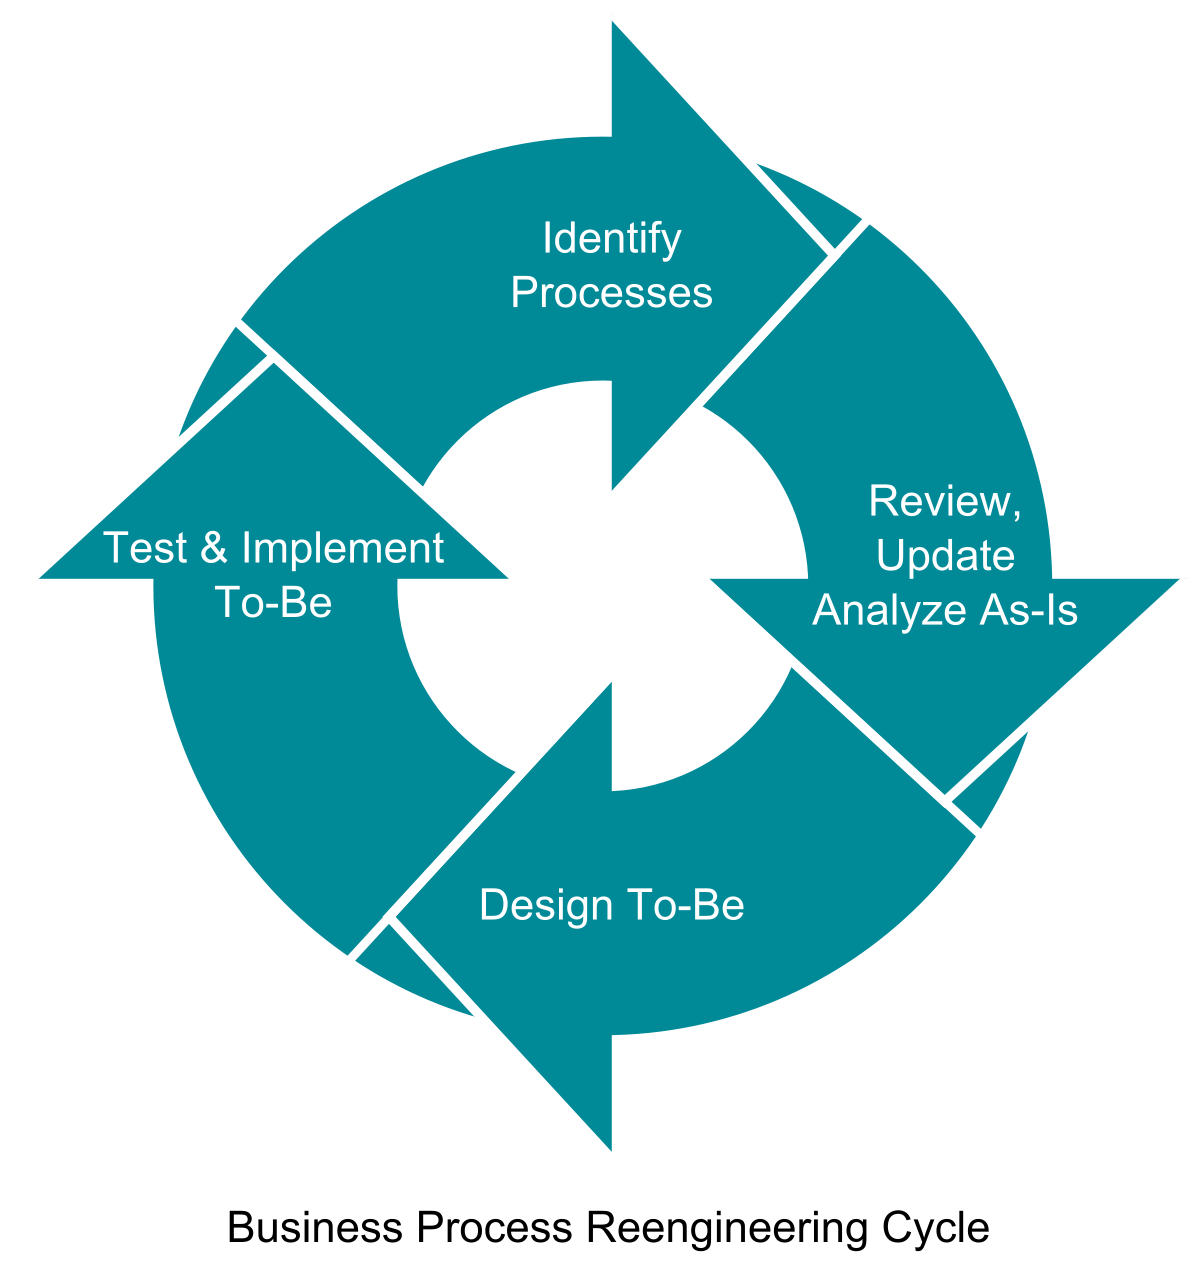
\includegraphics[width=\linewidth-2cm]{img/bpr}
			\caption{``\textit{Business process re-engineering cycle}''\cite{bpr}}
			\label{fig:bpr}
		\end{figure}
	
		L'attività di BPR può essere suddivisa in quattro fasi, come in Fig.~\ref{fig:bpr}:
		\begin{enumerate}
			\item \textit{Identificazione dei processi} (\textit{Identify Processes}): durante questa fase è necessario identificare i processi esistenti (\textit{as-is}) per avere le informazioni di base da cui partire;
			\item \textit{Revisione, aggiornamento e analisi dell’as-is} (Review, Update, Analyze As-is): in questa fase è necessario analizzare in profondità i processi identificati, allo scopo di avere più informazioni possibili;
			\item \textit{Design to-be}: in questa fase vengono progettati i nuovi processi, seguendo le linee guida e gli obiettivi del \proponente;
			\item \textit{Test e implementazione del to-be} (Test \& Implement To-Be): in quest’ultima fase i processi vengono testati ed effettivamente implementati nella realtà aziendale del \proponente.
		\end{enumerate}

		Per l'implementazione da parte di \azienda~si rimanda il lettore al paragrafo \ref{subsec:bpr_implmentation}.